%----------------------------------------------------------------------------------------
%	PACKAGES AND OTHER DOCUMENT CONFIGURATIONS
%----------------------------------------------------------------------------------------

\documentclass{article}

\usepackage{fancyhdr} % Required for custom headers
\usepackage{lastpage} % Required to determine the last page for the footer
\usepackage{extramarks} % Required for headers and footers
\usepackage[usenames,dvipsnames]{color} % Required for custom colors
\usepackage{graphicx} % Required to insert images
\usepackage{listings} % Required for insertion of code
\usepackage{courier} % Required for the courier font
\usepackage{lipsum} % Used for inserting dummy 'Lorem ipsum' text into the template
\usepackage{parskip}
% Margins
\topmargin=-0.45in
\evensidemargin=0in
\oddsidemargin=0in
\textwidth=6.5in
\textheight=9.0in
\headsep=0.25in

\linespread{1.1} % Line spacing

% Set up the header and footer
\pagestyle{fancy}
\chead{} % Top left header
\lhead{\hmwkClass\  \hmwkTitle} % Top center head
\rhead{} % Top right header
\lfoot{\lastxmark} % Bottom left footer
\cfoot{} % Bottom center footer
\rfoot{Page\ \thepage\ of\ \protect\pageref{LastPage}} % Bottom right footer
\renewcommand\headrulewidth{0.4pt} % Size of the header rule
\renewcommand\footrulewidth{0.4pt} % Size of the footer rule

\setlength\parindent{0pt} % Removes all indentation from paragraphs

%----------------------------------------------------------------------------------------
%	CODE INCLUSION CONFIGURATION
%----------------------------------------------------------------------------------------

% \definecolor{MyDarkGreen}{rgb}{0.0,0.4,0.0} % This is the color used for comments
\lstloadlanguages{C} % Load C syntax for listings, for a list of other languages supported see: ftp://ftp.tex.ac.uk/tex-archive/macros/latex/contrib/listings/listings.pdf
\lstset{language=C,commentstyle=\color{Green},frame=single,keywordstyle=[1]\color{Blue}\bf} % Use C in this example      



\newcommand{\csnippet}[2]{
\begin{itemize}
\item[]\lstinputlisting[caption=#2,label=#1]{#1.c}
\end{itemize}
}

%----------------------------------------------------------------------------------------
%	DOCUMENT STRUCTURE COMMANDS
%----------------------------------------------------------------------------------------

% Header and footer for when a page split occurs within a problem environment
\newcommand{\enterProblemHeader}[1]{
\nobreak\extramarks{#1}{#1 continued on next page\ldots}\nobreak
\nobreak\extramarks{#1 (continued)}{#1 continued on next page\ldots}\nobreak
}

% Header and footer for when a page split occurs between problem environments
\newcommand{\exitProblemHeader}[1]{
\nobreak\extramarks{#1 (continued)}{#1 continued on next page\ldots}\nobreak
\nobreak\extramarks{#1}{}\nobreak
}

\setcounter{secnumdepth}{0} % Removes default section numbers
\newcounter{homeworkProblemCounter} % Creates a counter to keep track of the number of problems

\newcommand{\homeworkProblemName}{}
\newenvironment{homeworkProblem}[1][Problem \arabic{homeworkProblemCounter}]{ % Makes a new environment called homeworkProblem which takes 1 argument (custom name) but the default is "Problem #"
\stepcounter{homeworkProblemCounter} % Increase counter for number of problems
\renewcommand{\homeworkProblemName}{#1} % Assign \homeworkProblemName the name of the problem
\section{\homeworkProblemName} % Make a section in the document with the custom problem count
\enterProblemHeader{\homeworkProblemName} % Header and footer within the environment
}{
\exitProblemHeader{\homeworkProblemName} % Header and footer after the environment
}

\newcommand{\problemAnswer}[1]{ % Defines the problem answer command with the content as the only argument
\noindent\framebox[\columnwidth][c]{\begin{minipage}{0.98\columnwidth}#1\end{minipage}} % Makes the box around the problem answer and puts the content inside
}

\newcommand{\homeworkSectionName}{}
\newenvironment{homeworkSection}[1]{ % New environment for sections within homework problems, takes 1 argument - the name of the section
\renewcommand{\homeworkSectionName}{#1} % Assign \homeworkSectionName to the name of the section from the environment argument
\subsection{\homeworkSectionName} % Make a subsection with the custom name of the subsection
\enterProblemHeader{\homeworkProblemName\ [\homeworkSectionName]} % Header and footer within the environment
}{
\enterProblemHeader{\homeworkProblemName} % Header and footer after the environment
}

%----------------------------------------------------------------------------------------
%	NAME AND CLASS SECTION
%----------------------------------------------------------------------------------------

\newcommand{\hmwkTitle}{Assignment\ \#5} % assignment title
\newcommand{\hmwkDueDate}{Monday,\ December\ 18,\ 2014} % due date
\newcommand{\hmwkClass}{Programming Concurrent Systems} % class
\newcommand{\hmwkClassTime}{} % lecture time
\newcommand{\hmwkClassInstructor}{} % lecturer
\newcommand{\hmwkAuthorName}{Alyssa - Ilias} %name

%----------------------------------------------------------------------------------------
%	TITLE PAGE
%----------------------------------------------------------------------------------------

\title{
\vspace{2in}
\textmd{\textbf{\hmwkClass:\ \hmwkTitle}}\\
\normalsize\vspace{0.1in}\small{Due\ on\ \hmwkDueDate}\\
\vspace{0.1in}\large{\textit{\hmwkClassInstructor\ \hmwkClassTime}}
\vspace{3in}
}

\author{\textbf{\hmwkAuthorName}}


%----------------------------------------------------------------------------------------

\begin{document}

\maketitle

%----------------------------------------------------------------------------------------
%	TABLE OF CONTENTS
%----------------------------------------------------------------------------------------

%\setcounter{tocdepth}{1} % Uncomment this line if you don't want subsections listed in the ToC

%\newpage
%\tableofcontents
\newpage

%----------------------------------------------------------------------------------------
%	Introduction
%----------------------------------------------------------------------------------------
\begin{homeworkProblem}[Introduction]

This assignment asked us to implement heat dissipation in Chapel and perform comparison experiments
with our previous implementations.


\end{homeworkProblem}
%----------------------------------------------------------------------------------------
%	Heat
%----------------------------------------------------------------------------------------

% To have just one problem per page, simply put a \clearpage after each problem

\begin{homeworkProblem}[Heat dissipation | Chapel]
\textbf{Solution description}

Our Chapel implementation is a pretty straight forward translation of the C reference 
code. The interesting part are the code segments which are parallelized by Chapel.

First let's inspect the main computation loop:

We used the forall keyword to point out that we want the outer loop parallelized. We also tried
using one forall ij loop but then we would have to loop through the matrix again in order to fix
the wrap-around columns, and compared to our current implementation is was slightly faster for
the 1000x1000 matrix but wouldn't scale well. 

\csnippet{main}{Main loop}

The reduction was far more complex than the computation loop as usual.
We came up with three different implementations: 
- The naive forall outer loop
- Chapel way to reduce
- Our custom reduce 

This is the segment of the winner (us ofcourse!) code:

\csnippet{reduce}{Reduction loop}

We left the other two implementation as commments in our code.

\textbf{Evaluation - Experiments}

We run our experiments on the DAS-4 system. We used a normal node which has 8 physical cores,
and used 8 threads, which we found to perform best in previous assignments.

The following graphs depict performance and walltime comparison overview without reductions.

The Chapel implementation has very poor performance compared to our openMP or pthread implementation.
On the other hand, the sequential version of Chapel is pretty competitive with the sequential version of C,
concerning performance.

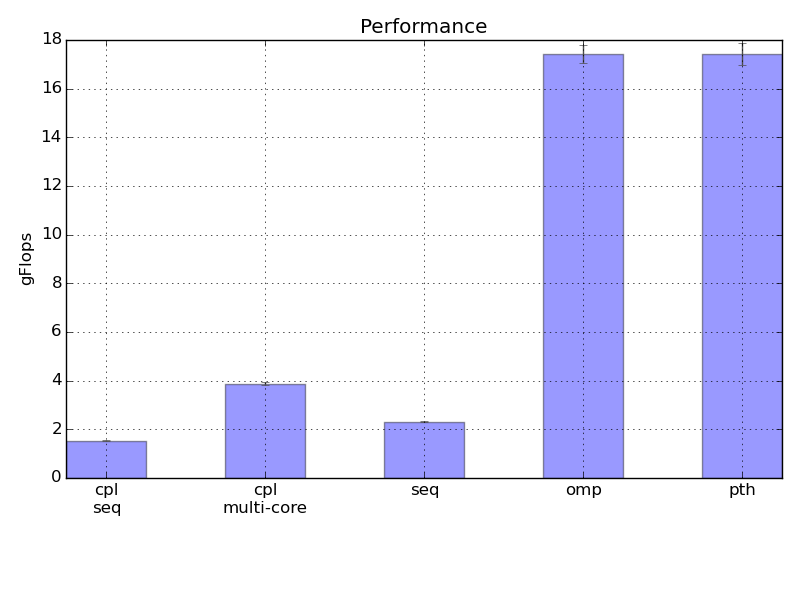
\includegraphics[width=0.75\columnwidth]{per_no_reductions.png} 

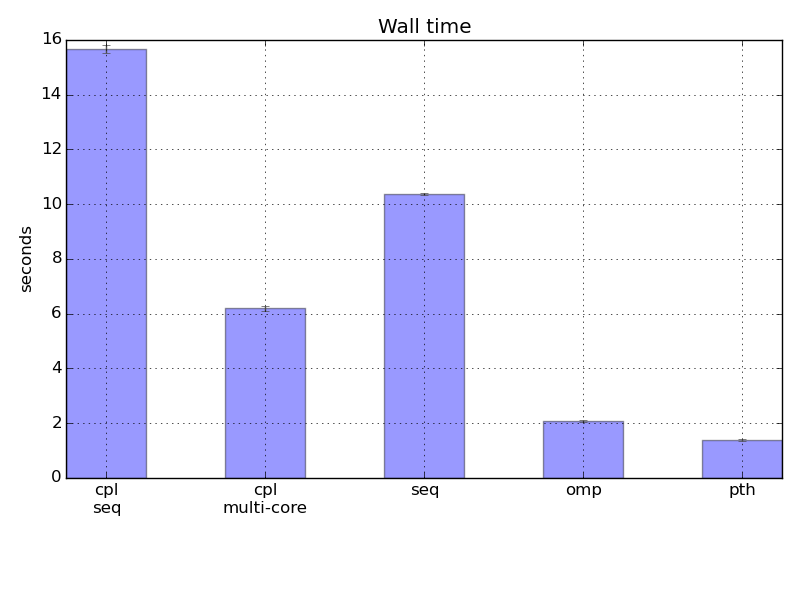
\includegraphics[width=0.75\columnwidth]{wt_no_reductions.png} 

Depiction of performance and walltime comparison overview with reductions.
We noticed that the performance of Chapel with or without reductions is almost the same which is a
result we didn't have on our earlier assignments concerning reductions. This might mean that the
parallelization of our main computation look might not be entierly optimized, or our reduction
implementation performs really well.

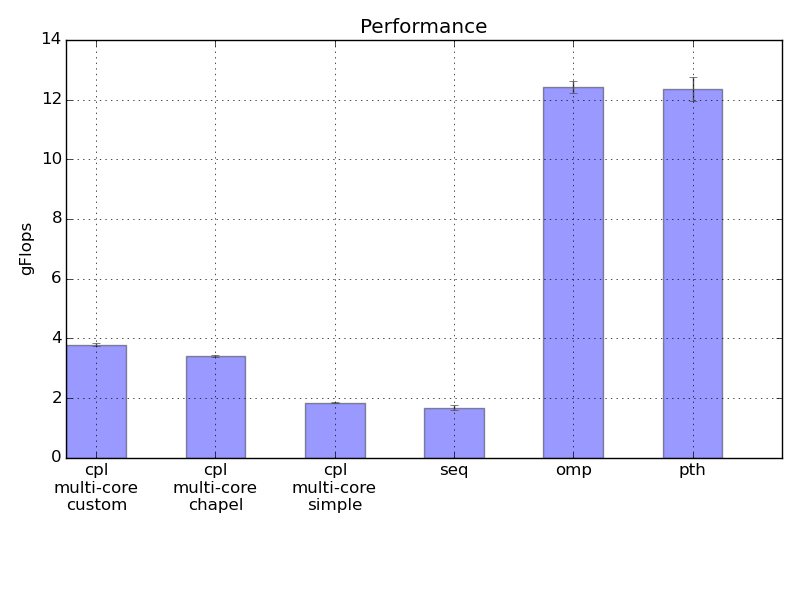
\includegraphics[width=0.75\columnwidth]{per_with_reductions.png} 

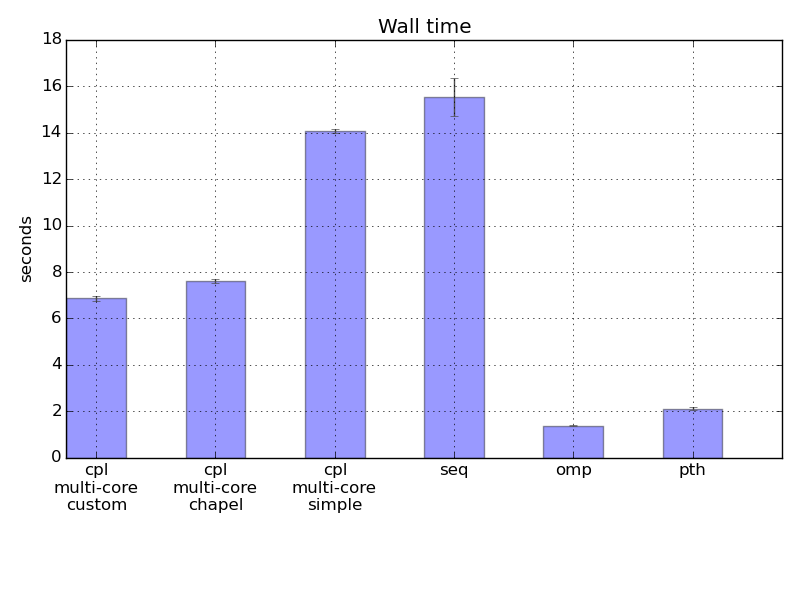
\includegraphics[width=0.75\columnwidth]{wt_with_reductions.png} 

Graph of different thread usage comparison without reductions. We can clearly see the performance
peak when all 8 threads are used. We also notice poor performance (non linear) when we
specify 4 threads. 

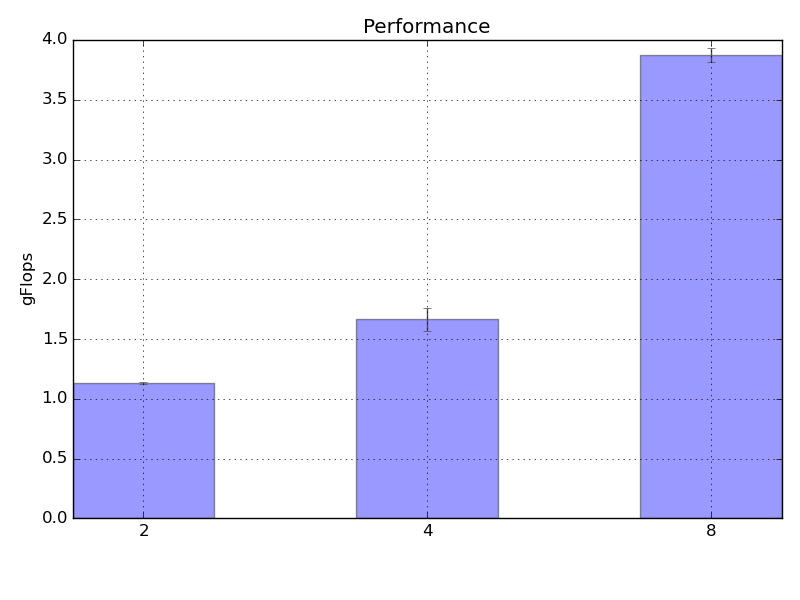
\includegraphics[width=0.75\columnwidth]{thread_without_reductions.png} 

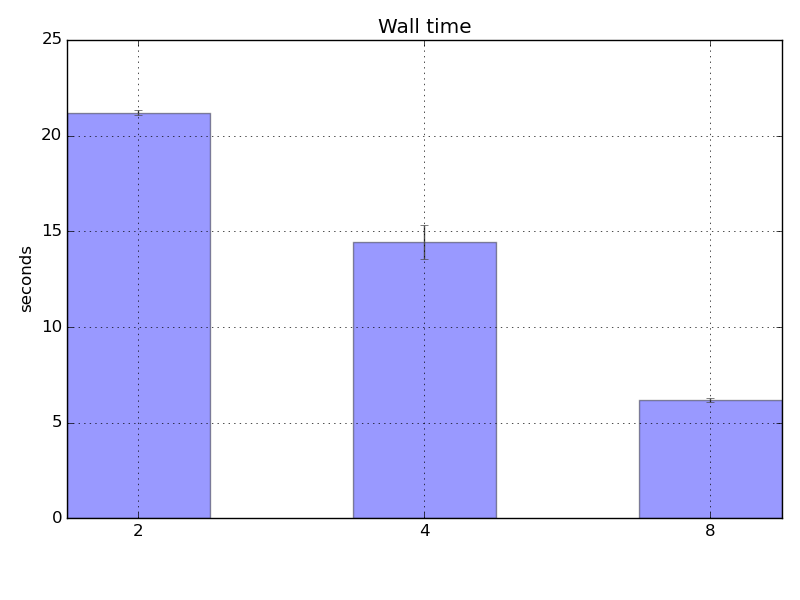
\includegraphics[width=0.75\columnwidth]{thread_without_reductions_wt.png} 

Graph of different thread usage comparison with reductions. Note that the reduction method
used is our custom reduction, which as shown above performed best. Equivelant results
as the ones without reductions.

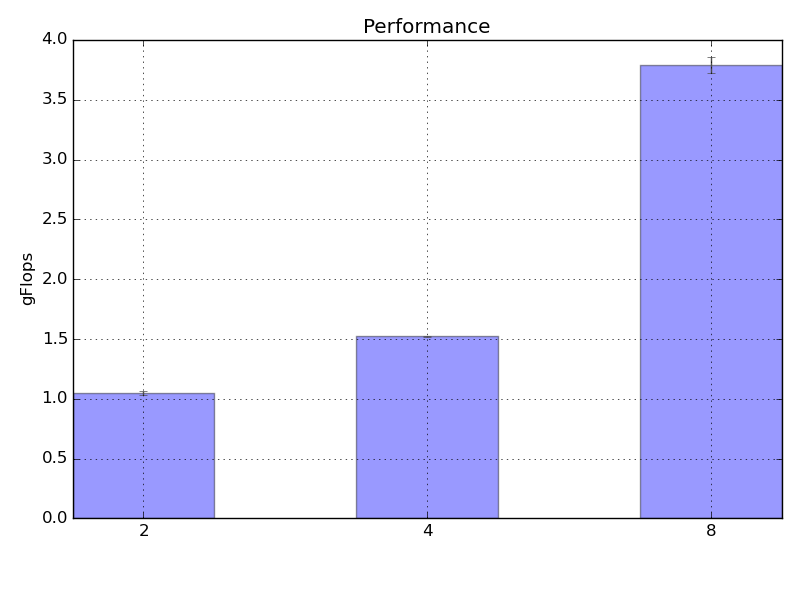
\includegraphics[width=0.75\columnwidth]{thread_with_reductions.png} 

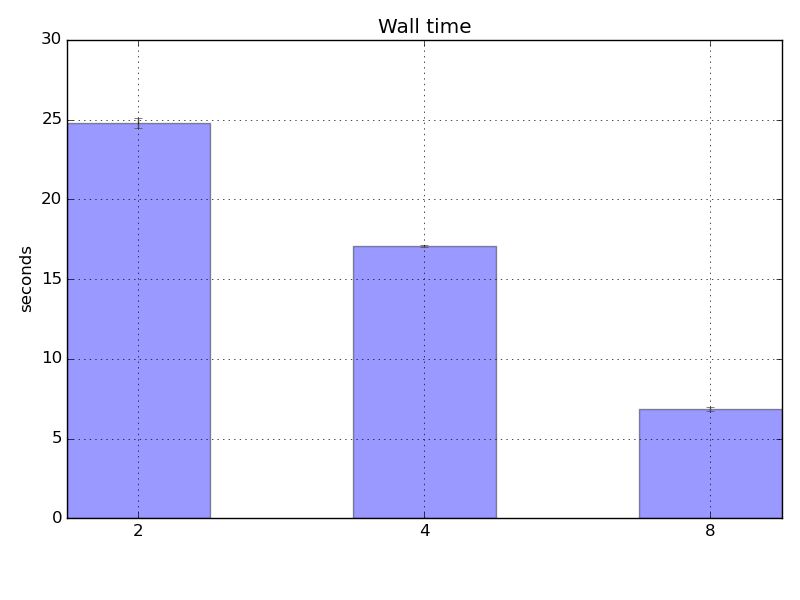
\includegraphics[width=0.75\columnwidth]{thread_with_reductions_wt.png} 


The experiments without were made with the following parameters:

\begin{verbatim}
./heat -e 0.0 -i 2000 -k 2001
\end{verbatim}

and with reduction:

\begin{verbatim}
./heat -e 0.0 -i 2000 -k 1
\end{verbatim}


\end{homeworkProblem}

\end{document}
